%Latex2e file
\documentclass[12pt,letterpaper]{article}
%\renewcommand{\arraystretch}{2}
%\input{\scrload.tex}
\setlength{\textwidth}{6.5in}
\setlength{\textheight}{8.6in}

\setlength{\oddsidemargin}{-.25in}
\setlength{\evensidemargin}{-.25in}
\setlength{\topmargin}{-.25in}
\pagestyle{empty}

\usepackage{amsmath}
\usepackage{amssymb}
\usepackage{graphicx}

\newcommand{\R}{\ensuremath{{\mathbb{R}}}}
\newcommand{\Z}{\ensuremath{{\mathbb{Z}}}}
\newcommand{\Q}{\ensuremath{{\mathbb{Q}}}}
\newcommand{\N}{\ensuremath{{\mathbb{N}}}}
\newcommand{\C}{\ensuremath{{\mathbb{C}}}}
\newcommand{\Proof}{\noindent {\bf Proof: }}
\newcommand{\QED}{\begin{flushright}QED\end{flushright}}
\newcommand{\Refl}{{\bf Reflexive: }}
\newcommand{\Symm}{{\bf Symmetric: }}
\newcommand{\Tran}{{\bf Transitive: }}
\newcommand{\ep}{\varepsilon}
\newcommand{\ri}{\right|}
\newcommand{\lef}{\left|}
\newcommand{\toR}{\to \R}
\newcommand{\fancy}[1]{#1_{\text{fancy}}}
\newcommand{\pro}[1]{\noindent {\bf #1}}
\newcommand{\prob}[1]{\newpage\noindent {\bf #1}}
\newcommand{\bacon}{\approx}

   
\begin{document}
\begin{flushright}
Nick Kerner

Homework 7

Chapter 6: 2, 3, 6, 7, 8, 12

Major Exercises 3, 11

\end{flushright}
\begin{center}
\large{Geometry}\\
\end{center}

\pro{2 }This problem has five parts.  In the first part we will construct Saccheri quadrilaterals associated with any triangle $\triangle ABC$.  Then we will apply this construction.  Figure 6.15 illustrates the case where the angles of the triangle at A and B are acute;  you are invited to draw the figure when one of these angles is obtuse or right.  \\


a. Let I,J,K be the midpoints of BC, CA, AB, respectively.  Let D, E, F, be the feet of the perpendiculars from A,B,C respectively, to $\overleftrightarrow{IJ}$ (which is called a medial line). \\ 


First I want to show somewhat obvious things, because a lot of proofs that follow depend on them.\\


By Exterior angle theorem, we know that if one angle is right or obtuse, then the other two are acute.\\



  

Lemma 1: First I prove that either E*I*F or E=I=F.

\Proof

\noindent Part 1: E*I*F\\

In order to show that E*I*F, we must first know that E,F, and I are three distinct points (we already know they are on the same line).  Assume to the contrary that two of the points are the same point, but the third is not.  So either E = F, E = I, or F = I. In each case we show that 

Case 1:  E = F
 
Assume to the contrary that $\overleftrightarrow{BF}$ and $\overleftrightarrow{CF}$ are distinct lines.  However $\overleftrightarrow{CE}$ and $\overleftrightarrow{CF}$ are both perpendicular to $\overleftrightarrow{EJ}$, so by Corollary 1 to the alternate interior angle theorem, we know that these two lines are parallel.  Therefore they do not intersect, however they intersect at E=F. Contradiction, then they are the same line.

Assume to the contrary that $E=F \neq I$.

Note that since  both $I \in \overleftrightarrow{BC}$ and $E\in \overleftrightarrow{EG}$, and we know that $I\in \overleftrightarrow{BC}$ and $E\in \overleftrightarrow{BC}$ so both $\overleftrightarrow{BC}$ and $I\in \overleftrightarrow{EG}$ could also be written as $\overleftrightarrow{EI}$, as this line is unique.  Additionally, we know that $J,C \in \overleftrightarrow{EI}$ and $J,C \in \overleftrightarrow{AC}$, so these two lines are the same line.  Therefore $\triangle ABC$ is not a triangle, it is a line. So triangles do not exist. Contradiction (I3 and definition of triangle).

Therefore E=F=C.


Case 2: E = I or F= I.  Note that both are the foot on $\overleftrightarrow{IJ}$ dropped from a vertex of a triangle.  We do not use the angle measure in this proof, so without loss of generality, let E=I.

Note that $E,I\in \overleftrightarrow{BC}$ by definition of I. So $\overleftrightarrow{BC}$ is perpendicular to $\overleftrightarrow{EJ}$ by definition of E.  We also know that $\overleftrightarrow{CF}$ is perpendicular to $\overleftrightarrow{IJ}$ by definition of F.  By an argument made on page 126, we know that the line ($\overleftrightarrow{BE},\overleftrightarrow{CF}$) perpendicular to another line $\overleftrightarrow{IJ}$ through a point not on that line (C) is unique.  So $\overleftrightarrow{BE}=\overleftrightarrow{CF}$.  By an argument similar to case 1 ($E,F\in \overleftrightarrow{IJ}$), triangles do not exist. Contradiction.


Therefore if all three points are not distinct from each other, E=F=I.\\

Now assume that the three points are distinct and note the possibilities.

E*I*F = F*I*E

I*E*F = F*E*I

E*F*I = U*F*E

Assume to the contrary that either I*E*F or E*F*I.  Note that we only use the facts that $\angle CFI$ and $\angle BEI$ are right angles, so without loss of generality, we show that $I*E*F $.

So we know that $\angle CFI$ is a right angle and that $\angle FIB^\circ = \angle CFI^\circ + \angle ICF^\circ$, so that means that neither other angle of $\triangle BIE$ can be obtuse or right.  However, $\angle BEI$ is a right angle.  Contradiction.  Therefore E*I*F if the three points are distinct. 

\QED




\newpage 


Prove, in any Hilbert plane, that $AD \cong CF \cong BE$, hence that $\square EDAB$ is a Saccheri quadrilateral with base ED summit AB.  \\


\Proof

First we show $CF \cong BE$\\

\noindent Case 1: $E \neq F \neq I$ \\

By the definition of midpoint we know that $BI \cong IC$ and $CJ \cong JA$.  Also, vertical angle pairs are congruent, so $\angle BIE \cong \angle CIE$ and $\angle AJD \cong CJF$.  By SAA we know then that $\triangle BIE \cong \triangle CIF$, so $BE \cong CF$ and again by SAA we know $\triangle ADJ \cong \triangle CJF$ so $CF \cong AD$.  Hence $AD \cong BE$. \\

Therefore $\square EDAB$ has two congruent opposite sides, $BE \cong AD$ and each are perpendicular to $\overleftrightarrow{ED}$, which meets our definition of a Saccheri quadrilateral. \\

\noindent Case 2: $E = F = I$ (previous proof demonstrated that these are the only two possibilities)\\

$BE = BI \cong IC = FC$ as I is the midpoint of BC.\\

Similarly, $CF \cong AD$, so $AD \cong CF \cong BE$.

\QED


\newpage

Show that a triangle and its associated Saccheri quadrilateral have equal content-- ie, that you can dissect the Saccheri quadrilateral region into polygonal pieces and then reassemble these pieces to construct the triangular region. \\



\Proof

Case 1: F = E or F= D.  Without loss of generality, let F = E.

We know from lemma 1 that F*J*D (unless F=J=D which would mean that A is collinear with B and C). So we know that A,D, and J are on the Saccheri quadrilateral, so the interior of this triangle will be interior to the quadrilateral (it is convex, J is interior to $\angle DAE$).  So we must find a triangle congruent to this outside of $\square EDAB$ but inside $\triangle ABC$.  Fortunately we have shown that $\triangle ADJ \cong \triangle CFJ$. The only remaining part of $\square EDAB$ to show is congruent to a part of $\triangle ABC$ is $\square EJAB$ which is part of both.


Case 2: E*F*D

So we know then that E*I*F*J*D.  So we know that $\triangle BEI\cong \triangle CFI$ and $\triangle CFJ \cong \triangle ADJ$, but $\triangle CFI$ and $\triangle CFJ$ are not in the quadrilateral, but are in $\triangle ABC$.  So this portion of area matches.  The only portion remaining to equate is $\square BIJA$, which is in both.  So the area of the Saccheri quadrilateral is equal to the area of $\triangle ABC$.\\


Case 3: F*E*D or F*D*E.  Without loss of generality, let $F*E*D$.

Subcase 1: E*J*D

Note that we have F*I*E*J*D, so $\square EJAB$ is contained in both. All we have left to show is in both is $\triangle ADJ$ and something congruent to it.  Fortunately we have shown that $\triangle ADJ \cong CFJ$.  However, part of $\triangle CFJ$ is not contained within either $\triangle ABC$ or the quadrilateral.  So we need another part of $\triangle ABC$ that this is congruent to. Fortunately, we have shown that $\triangle BEI \cong \triangle CFI$. 

Subcase 2: J*E*D

Note that I*J*D as $FI\cong IE$ and $FJ \cong JD$ so the distance from F to I is $\frac{1}{2}FE$ and the distance from F to J is $\frac{1}{2}FD$ where F*E*D.

There is a point where BE intersects AC.  Call it Q. note that BE and AD are both perpendicular to ED, so they are parallel.  So A and D are on the same side of $\overleftrightarrow{BE}$.  D and J are on opposite sides of $\overleftrightarrow{BE}$ as J*E*D. So J and A are on opposite sides of $\overleftrightarrow{BE}$, however, Q lies on BE so J*Q*A.  Also, J is on $\overleftrightarrow{IJ}$ but in the opposite direction from D starting at E.  So $\triangle JQE$ is not contained in $\square EDAB$. 

Note that $\triangle ABQ$ is contained in the quadrilateral.  However, we must also include the portion of $\triangle ADJ$ that is.



So $\overrightarrow{AQ}$ intersects $\overleftrightarrow{IJ}$ at J, but D and A are on the same side o

\begin{eqnarray*}
\square EDAB &=& \triangle BAQ + (\triangle ADJ - \triangle JQE)\\
&=& \triangle BAQ + \triangle CFJ - \triangle JQE\\
&=& \triangle BAQ + \triangle CIJ + \triangle CFI - \triangle JQE\\
&=& \triangle BAQ + \triangle CIJ + (\triangle BEI - \triangle JQE)\\
&=& \triangle ABC
\end{eqnarray*}

Note, there is technically also a subcase when J = E, but this will merely give $\triangle JQE$ no area.  The math still works with that information. 

\QED





\newpage 

b. Prove that the perpendicular bisector of AB is also perpendicular to $\overleftrightarrow{IJ}$. (Hint: Use a result about Saccheri quadrilaterals.)  Hence if the plane is hyperbolic, $\overleftrightarrow{IJ}$ is divergently parallel to $\overleftrightarrow{AB}$.  Assume now the plane is real, so lengths can be assigned (Theorem 4.3) and the Saccheri-Legendre theorem applies. \\

\Proof

As we have a Saccheri quadrilateral, we know that $EB \cong DA$ and $\angle EBK \cong \angle DAK$.  Additionally, by our definition of K, we know that $BK \cong AK$.  Therefore by SAS we know that $\triangle EBK \cong \triangle DAK$.  So $EK \cong DK$ and $\angle BKE \cong \angle AKD$.  Next consider the perpendicular bisector of AB.  Say there is some point on it Z such that Z and C are on the same side of $\overleftrightarrow{BA}$, so $\angle BKZ \cong \angle AKZ$. \\

Note that since $\angle AKD \cong \angle BKE$ and since we know that B and D are distinct points, we know that they are acute angles (they do not make right angles, as that would require E=D, but they are congruent to each other). So we know that $\overrightarrow{KZ}$ is between $\overrightarrow{KE}$ and $\overrightarrow{KD}$.  By the crossbar theorem, we know that $\overrightarrow{KZ}$ intersects ED, call this point K'.\\

So consider $\triangle EKD$.  We now know that this is isosceles so $\angle KED \cong \angle KDE$. Additionally we know that since $\angle BKK' \cong \angle AKK'$ and $\angle BKE \cong \angle AKD$ that $\angle EKK' \cong  DKK'$ by angle subtraction.  So by ASA, we know that $\triangle KEK' \cong\triangle KDK'$.  Therefore $\angle EK'K \cong \angle DK'K$ so they are right angles, that is, $\overleftrightarrow{KK'}$ is perpendicular to $\overleftrightarrow{ED} = \overleftrightarrow{IJ}$. 



\QED







\newpage 

c. Prove that $\overline{ED} = 2\overline{IJ}$.  Deduce that $\overline{AB} > 2\overline{IJ}$ (respectively $\overline{AB} = 2\overline{IJ}$) if the plane is hyperbolic (respectively is Euclidean).\\

\Proof


Case 1: I*F*J

By segment addition we know that $IJ = IF + FJ$ and we know that $ED = EI + IF + FJ + JD$.  Additionally, in an early part of the problem we showed that $\triangle EBI \cong \triangle FCI$ and $\triangle CFJ \cong \triangle ADJ$.  So we know that $EI \cong IF$ and $FJ \cong JD$.  Therefore 

\begin{eqnarray*}
ED &=& EI + IF + FJ + JD\\
&=& IF + IF + FJ + FJ\\
&=& (IF + FJ) + (IF + FJ)\\
&=& 2(IF + FJ)\\
&=& 2IJ
\end{eqnarray*}

Case 2: F=I or F=J.  Without loss of generality, let F=I. 

So F=I=E.  So we know that F*J*D, so ED = IJ + JD, and we know by congruent triangles that IJ = JD, so ED = IJ + IJ = 2IJ.

Case 3:  F*I*E*J*D

So we know that ED = EJ + JD and we know that FI = IE and FJ = JD (congruent triangles, again).  Also IE + EJ = IJ.  So 

\begin{eqnarray*}
ED &=& EJ + JD\\
&=& EJ + FJ \\
&=& EJ + FI + IJ\\
&=& EJ + IE + IJ\\
&=& IJ + IJ\\
&=& 2IJ\\
\end{eqnarray*}


Case 4: F*I*J*E*D

We also showed that FI < FJ so F*I*J. 

\begin{eqnarray*}
ED &=& JD - JE\\
&=& FI + IJ -JE\\
&=& IJ + IE - JE\\
&=& IJ + IJ\\
&=& 2IJ\\
\end{eqnarray*}


Case 5: F*I*J=E*D

Note that by congruent triangles, we knew earlier that $FJ \cong JD$.  

\begin{eqnarray*}
ED &=& FJ \\
&=& FI + IJ \\
&=& IE + IJ \\
&=& IJ + IJ\\
&=& 2IJ
\end{eqnarray*}

\QED


If the plane is hyperbolic, then we know that by theorem 6.2 that the acute angle hypothesis is satisfied, so by Corollary 4 to Saccheri III, we know that the summit of $\square BADE$ (BA) is greater than the base (ED).  Therefore $AB > ED = 2IJ$.  

Similarly, if in Euclidean geometry, $\square ABDE$ is a rectangle, and by Corollary 4 to Saccheri III, the base is equal to the summit.  Therefore $AB = ED = 2IJ$.  






\newpage 

d. Prove that K,F, and C are collinear if and only if $AC \cong BC$ (isosceles triangle).  If that is the case, prove that F is the midpoint of CK iff the plane is Euclidean.  If K,F, and C are not collinear and the plane is not Euclidean, prove that F is the midpoint of CK iff the plane is Euclidean.  If K, F, and C are not collinear and the plane is not Euclidean, prove that $\overline{CF}$ is not perpendicular to $\overline{AB}$ (ray $\overrightarrow{CF}$ does intersect AB at some point G in the case shown, where the angles at A and B are acute, by the crossbar theorem, but CG is not an altitude of the triangle if the plane is not Euclidean).\\

Prove that K,F, and C are collinear iff $AC \cong BC$\\

\Proof

$\Rightarrow:$  Assume K, F, and C are collinear.

We know that the perpendicular bisector of AB through K is perpendicular to $\overleftrightarrow{IJ}$, but we also know that K,F, and C are collinear, but the line through C and F is perpendicular to IJ, so either we have found two points through K both perpendicular to $\overleftrightarrow{IJ}$ or they are the same line.  But we can only have 1 (pg 126), so they are the same line.  So we know that $AK\cong BK$ and $KC \cong KC$ and since $KC$ is part of the perpendicular bisector of AB, $\angle AKC \cong \angle BKC$ so by SAS $\triangle AKC \cong \triangle BKC$. So we know that $AC \cong BC$.


$\Leftarrow:$  Assume $AC \cong BC$.  

So we know that $AK \cong BK$ by the definition of K, and we know that $KC \cong KC$ by an axiom. So $\triangle ABC$ is isosceles, so $\angle CBA \cong \angle CAB$.  So by SAS we know that $\triangle BKC \cong \triangle KAC$ ($BK \cong KA$ by definition of K).  Therefore we know that $\angle BCK \cong \angle ACK$, so $\overleftrightarrow{CK}$ is the perpendicular bisector of AB. Now we have shown that the perpendicular bisector of AB is also perpendicular to $\overleftrightarrow{IJ}$, so if we assume $\overleftrightarrow{CK}$ and $\overleftrightarrow{CF}$ are distinct then we now have 2 lines through C both perpendicular to $\overleftrightarrow{IJ}$.  Contradiction (pg 126).  So they are the same line.  Hence C,K, and F are collinear. 


\QED







\newpage 

e. Show that if the Pythagorean equation holds for all right triangles and if $\angle C$ is a right angle, then $\overline{AB} = 2\overline{IJ}$ can be proved.  Deduce from part c that such a plane must be Euclidean.  (Use these results to add to your answers in Exercise 1.)

Assume that the Pythagorean equation holds for all right triangles and $\angle C$ is a right angle.

\begin{eqnarray*}
\overline{AB} &=& \sqrt{\overline{CA}^2 + \overline{CB}^2}\\
&=& \sqrt{(\overline{CJ} + \overline{JA})^2 + (\overline{CI} + \overline{IB})^2}\\
&=& \sqrt{\overline{CJ}^2 + 2\overline{CJ} \overline{JA} + \overline{JA}^2 +\overline{CI}^2 + 2\overline{CI} \overline{IB} + \overline{IB}^2}\\
&=& \sqrt{\overline{CJ}^2 + 2\overline{CJ} \overline{CJ} + \overline{CJ}^2 +\overline{CI}^2 + 2\overline{CI} \overline{CI} + \overline{CI}^2}\\
&=& \sqrt{4\overline{CJ}^2 + 4\overline{CI}^2}\\
&=& \sqrt{4(\overline{CJ}^2 + \overline{CI}^2)}\\
&=& 2\sqrt{\overline{CJ}^2 + \overline{CI}^2}\\
&=& 2 IJ
\end{eqnarray*}


Hence from part c we know that if this is the case then we cannot be hyperbolic, because that would mean that $\overline{AB} > 2\overline{IJ}$.






\prob{3 }(Hyperbolic geometry)
Assume that parallel lines l and l' have a common perpendicular segment MM'.  Prove that MM'  is the shortest segment between any point of l and any point of l'.  (Hint: In showing $MM' < AA'$, first dispose of the case in which A' is perpendicular to l' by means of a result about Lambert quadrilaterals and then take care of the other case by Exercise 22, chapter 4.)

\Proof

Given some other point A on l, drop a foot to l' and call it A'.  So we know that $\angle AMM', \angle A'M'M,$ and $\angle MAA'$ are right angles, so $\square AMM'A'$ is a Lambert quadrilateral.  Since we are hyperbolic, the fourth angle must be acute.  By Saccheri III we know that the sides adjacent to $\angle AA'M'$ are greater than the sides opposite them.  Hence $MM' < AA'$ and $MA < M'A'$.

\QED






\prob{6 }Let $\overrightarrow{PY}$ be a limiting parallel ray to  through P and let X be a point on this ray between P and Y (Figure 6.17).  It may seem intuitively obvious that $\overrightarrow{XY}$ is a limiting parallel ray to l through X, but this requires proof.  Justify the steps that have not been justified. 

1. We must prove that any ray $\overrightarrow{XS}$ between $\overrightarrow{XY}$ and $\overrightarrow{XR}$ meets l, where R is the foot of the perpendicular from X to l. 

This is part of the definition of limiting parallel rays.  It just says what we need to prove.\\



2. S and Y are on the same side of $\overrightarrow{XR}$.  

By definition, $\overrightarrow{XS}$ is between $\overrightarrow{XY}$ and $\overrightarrow{XR}$, so S is on the interior of $\angle RXY$.  So by definition of a point being interior to an angle, S and Y are on the same side of $\overleftrightarrow{XR}$. \\


3. P and Y are on opposite sides of $\overleftrightarrow{XR}$. 

By the problem statement we know that P*X*Y, so PY intersects $\overleftrightarrow{XR}$ at X, so P and Y are on opposite sides of this line.\\

4. By Exercise 5, S and Y are on the same side of $\overleftrightarrow{PQ}$.  

By part 3 we know that P and Y are on opposite sides of $\overleftrightarrow{XR}$, so by part 2 we know that S and P are on opposite sides of $\overleftrightarrow{XR}$. So S and Y are on the opposite side of $\overleftrightarrow{XR}$ from $\overleftrightarrow{PQ}$, so S and Y are on the same side of $\overleftrightarrow{PQ}$ (result from problem 5).\\


5. S and R are on the same side of $\overleftrightarrow{XY} = \overleftrightarrow{PY}.$

By definition, $\overrightarrow{XS}$ is between $\overrightarrow{XY}$ and $\overrightarrow{XR}$.  So we know that S and R  are on the same side of $\overrightarrow{XY}$ as S is interior to $\angle RXY$ and that is the definition of interior point.\\


6. Q and R are on the same side of $\overleftrightarrow{PY}$.

Assume to the contrary that they are not.  So QR intersects $\overleftrightarrow{PY}$. But $\overleftrightarrow{PY}$ and $\overleftrightarrow{QR}$ do not intersect (definition of limiting parallel rays).  Contradiction.  So Q and R are on the same side of $\overleftrightarrow{PY}$. \\


7. Q and S are on the same side of $\overleftrightarrow{PY}$.

Q and R are on the same side of $\overleftrightarrow{PY}$ and R and S are on the same side of $\overleftrightarrow{PY}$ so Q and S are on the same side of $\overleftrightarrow{PY}$. \\


8. Thus, $\overrightarrow{PS}$ lies between $\overrightarrow{PY} $ and $\overrightarrow{PQ}$, so it intersects l in a point T.  

Since Q and S are on the same side of $\overleftrightarrow{PY}$ and S and Y are on the same side of $\overleftrightarrow{PQ}$, we know that S is interior to $\angle YPQ$. so $\overrightarrow{PS}$ is between $\overrightarrow{PY} $ and $\overrightarrow{PQ}$.  It intersects by definition of limiting parallel rays ($\overrightarrow{PY}$ is one).\



9. Point X is exterior to $\triangle PQT$.  

Assume to the contrary that it is interior to the triangle.  So it is on the interior of $\angle TPQ$, so by proposition 3.9a, $\overrightarrow{PX} = \overrightarrow{PY}$ must intersect QT which is part of $\overleftrightarrow{QT}$.  Contradiction as this is a limiting parallel ray to that line. \\



10. $\overrightarrow{XS}$ does not intersect PQ.  

$\overrightarrow{XS}$ is between $\overrightarrow{XR}$ and $\overrightarrow{XY}$, so S in on the interior of $\angle YXR$ so by Proposition 3.8 we know that every other point on $\overrightarrow{XS}$ is as well.  So every point on $\overrightarrow{XS}$ is on the same side of $\overleftrightarrow{XR}$ as Y, which we know to be on the opposite side of $\overleftrightarrow{XR}$ as $\overleftrightarrow{PQ}$.  So the ray and line cannot intersect, so the ray cannot intersect the segment PQ either. 



11. Hence $\overrightarrow{XS}$ intersects QT (proposition 3.9a), so $\overrightarrow{XS}$ meets l. 

We know that $\overrightarrow{XS}$ intersects PT as $P*S*T$, and we know it does not intersect PQ, so by proposition 3.9a, $\overrightarrow{XS}$ intersects QT.




\prob{7 } Let us assume instead that $\overrightarrow{XY}$ is limiting parallel to l, with P*X*Y.  Prove that $\overrightarrow{PY}$ is limiting parallel to l.  (Hint: See figure 6.18.  You must show that $\overrightarrow{PZ}$ meets l in a point V.  Choose any S such that S*P*Z.  Show that SX meets $\overleftrightarrow{PQ}$ in a point U such that U*P*Q.  Choose any W such that U*X*W and show that $\overrightarrow{XW}$ is between $\overrightarrow{XY}$ and $\overrightarrow{XR}$ so that $\overrightarrow{XW}$ meets l in a point T.  Apply Proposition 3.9(a) to get V.)

\Proof


Given an arbitrary ray $\overrightarrow{PZ}$ between $\overrightarrow{PQ}$ and $\overrightarrow{PY}$.  We also know by B2 that there is some point S such that $S*P*Z$. Since Z is an interior point of $\angle QPX$ we know that X and Z are on the same side of $\overleftrightarrow{PQ}$.  Additionally, since S*P*Z we know that S and Z are on opposite sides of  $\overleftrightarrow{PQ}$.  So S and X are on opposite sides of $\overleftrightarrow{PQ}$.  Therefore SX intersects $\overleftrightarrow{PQ}$ at some point, call it U (note that S*U*X).  \\

So Z and Q on the same side of $\overleftrightarrow{PX}$ by the definition of Z (interior point of $\angle QPX$), but S and Z are on opposite sides of $\overleftrightarrow{PX}$ (SZ intersected it at P), so S and Q are on opposite sides of $\overleftrightarrow{PX}$.  Additionally, we know that S*U*X, so U and S are on the same side of $\overleftrightarrow{PX}$ (SX can only intersect $\overleftrightarrow{PX}$ once and it does this at X, if it intersected it more than once then $\overleftrightarrow{PX} = \overleftrightarrow{SX}$ which means that either S = P or $\overleftrightarrow{PZ} = \overleftrightarrow{PX}$, however, Z is interior to $\angle QPX$ and S*P*Z). This means that U and Q are on opposite sides of $\overleftrightarrow{PX}$, so U*P*Q.\\


Given some point W such that U*X*W, we note that R and Q are on a line parallel to $\overleftrightarrow{PX}$ so they are on the same side of $\overleftrightarrow{PX}$, and we know that U and Q are on opposite sides of $\overleftrightarrow{PX}$, and since U*X*W we know that U and W are on opposite sides of $\overleftrightarrow{PX}$.  Therefore W and Q are on the same side of $\overleftrightarrow{PX}$, so W and R are on the same side of $\overleftrightarrow{PX}$.  \\

Note that since UW intersects $\overleftrightarrow{XR}$ at X, U and W are on opposite sides of $\overleftrightarrow{XR}$.  Similarly we know that P and Y are on opposite sides of $\overleftrightarrow{XR}$.  \\





Note that since $\overleftrightarrow{PR}$ and $\overleftrightarrow{PQ}$ make right angles to l, they are parallel, ie they are not the same line.  If they were, either P=X or $\overleftrightarrow{XR} = \overleftrightarrow{PX}$, both of which are contradictions (one means they are parallel but they intersect at X, and we assumed they were different points in the problem statement). So U and P are on the same side of $\overleftrightarrow{XR}$ ($\overleftrightarrow{UPQ}$ and $\overleftrightarrow{XR}$ are parallel), so W and P are on opposite sides of $\overleftrightarrow{XR}$ and therefore W and Y are on the same side of $\overleftrightarrow{XR}$.  Therefore W is on the interior of $\angle RXY$ so $\overrightarrow{XW}$ is between $\overrightarrow{XR}$ and $\overrightarrow{XW}$, so since $\overrightarrow{XY}$ is a limiting parallel to l, $\overrightarrow{XW}$ must intersect l, call this point T.\\


Consider $\triangle UQT$. So since we know that $\overrightarrow{SZ}$ intersects UQ at P, and since it can only intersect $\overleftrightarrow{ST}$ at S, it does not intersect UT. So by Proposition 3.9a, it must intersect QT. Since $\overrightarrow{SZ} = \overrightarrow{PZ}$ was an arbitrary ray between $\overrightarrow{PQ}$ and $\overrightarrow{PY}$, this means that $\overrightarrow{PY}$ is a limiting parallel ray to l.


\QED







\prob{8 } Let $\overrightarrow{PX}$ be the right limiting parallel ray to l through P and let Q and X' be the feet of the perpendiculars from P and X, respectively, to l (Figure 6.19).  Prove that PQ > XX'. (Hint: Use Exercise 6 to show that $\angle X'XY$ is acute and that $\angle X'XP$ is obtuse, so that Proposition 4.13, Chapter 4, can be applied to $\square PQX'X$.) This exercise shows that the distance from X to l decreases as X recedes from P along a limiting parallel ray.  In fact, on e can prove that the distance from X to l approaches zero (see Major exercise 11).

\Proof

By Exercise 6 we know that $\overrightarrow{XY}$ (Where Y is arbitrary such that P*X*Y) is a limiting parallel to l and by proposition 6.6 we know that $\angle X'XY$ is acute.  However, it is supplementary to $\angle X'XP$ so $\angle X'XP$ is obtuse.  Also by proposition 6.6 we know that $\angle QPX$ is acute.  So by proposition 4.13 we know that in the bi-right quadrilateral $\square QX'XP$ that the greater side is opposite the greater summit angle.  Therefore $\angle X'XP$ is the greater summit angle so $PQ$ is the greater side.  Hence $ PQ > XX'$.

\QED








\prob{12 } In theorem 4.1 it was proved in neutral geometry that if alternate interior angles are congruent, then the lines are parallel.  Strengthen this result in hyperbolic geometry by proving that the lines are divergently parallel, ie, that they have a common perpendicular.  (Hint: Let M be the midpoint of transversal segment PQ and drop perpendiculars MN and ML to lines m and l;  see Figure 6.23.  Prove that L, M, and N are collinear by the method of congruent triangles.)


\Proof

Suppose we have two lines m and l and a transversal t such that a pair of alternate interior angles are congruent.   Call the place where t meets m P and call the place where t meets l Q.  Call the midpoint of PQ M. \\

\noindent Case 1: The alternate interior angles are right angles. \\

We are done.\\

\noindent Case 2: They are not.\\

Let N be the foot of the perpendicular from M to m and let L be the foot from M to l.    \\

So we know that $\angle P \cong \angle Q$, $QM \cong MP$ and $\angle MLQ \cong \angle MNP$, so by ASA we know that $\triangle LMQ \cong \triangle NMP$. So $\angle QML \cong \angle PMN$.  Also we know that 
\begin{eqnarray*}
180^\circ &=& \angle QMN^\circ + \angle NMP^\circ\\
&=& \angle QMN^\circ + \angle LMQ^\circ
\end{eqnarray*}

So $\angle QMN$ and $\angle LMQ$ are supplementary, share a ray and their vertex, so $N,M,$ and $L$ are collinear.  Therefore $\overleftrightarrow{NL}$ is perpendicular to both m and l, so we have found a common perpendicular.  

\begin{center}
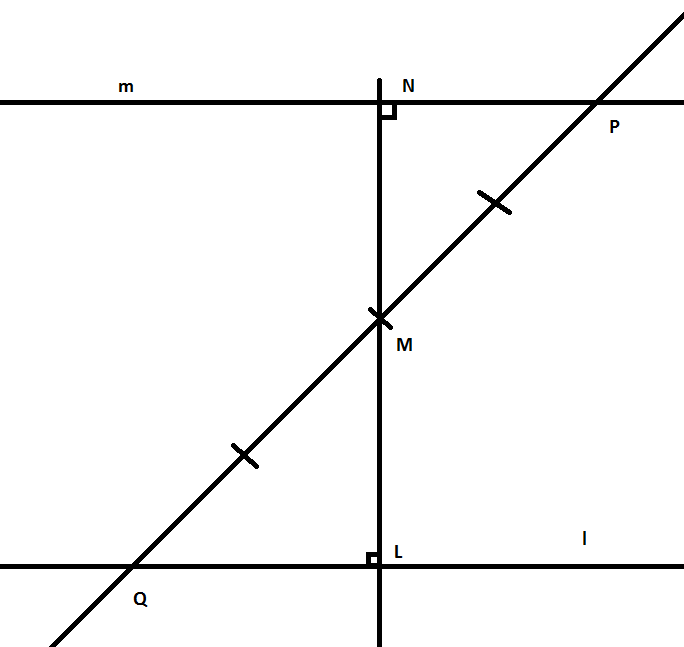
\includegraphics[width=2in]{perpendiculars.png}
\end{center}

\QED





\prob{Major Exercises 3 }

Transitivity of limiting parallelism.  If $\overrightarrow{AB}$ and $\overrightarrow{CD}$ are both limiting parallel to $\overrightarrow{EF}$, then they are limiting parallel to each other. Justify the steps in the proof.  \\

1. $\overleftrightarrow{AB}$ and $\overleftrightarrow{CD}$ have no point in common.\\

Of course what is meant by the problem statement is that the lines are distinct, so what needs to be shown here is that they do not have exactly 1 point in common (we already know that they do not have 2, as they would not be distinct).\\

Assume to the contrary that $\overleftrightarrow{AB}$ and $\overleftrightarrow{CD}$ have a point in common, call this point X.  By exercise 6 we know we can find limiting parallels $\overrightarrow{XY} \subset \overleftrightarrow{AB}$ and $\overrightarrow{XZ} \subset \overleftrightarrow{CD}$.\\

Let V be the foot of X to $\overleftrightarrow{EF}$ (if this does not exist, then we do not have a limiting parallel ray, which would contradict exercise 6).  By exercise 6 we know that $\overrightarrow{XY}$ and $\overrightarrow{XZ}$ are limiting parallel rays to $\overrightarrow{EF}$. By proposition 6.6 we know that either they are the same ray (contradiction, problem statement) or Y and Z are on opposite sides of $\overleftrightarrow{XV}$.  Without loss of generality let E and Y be on the same side of $\overleftrightarrow{XV}$.\\


Note that our original limiting parallel ray was a limiting parallel to $\overrightarrow{EF}$ but it is possible that V*E*F or E=V, which would mean that if both of our limiting parallel rays $\overrightarrow{AB}$ and $\overrightarrow{CD}$ are limiting parallel to $\overrightarrow{EF}$ then our new limiting parallels $\overrightarrow{XZ}$ and $\overrightarrow{XY}$ will be limiting to $\overrightarrow{VF}$, but only if V*E*F.  Also note that if V*E*F, then any ray between $\overrightarrow{XZ}$ and $\overrightarrow{XV}$ will intersect $\overleftrightarrow{EF}$ but not $\overrightarrow{VF}$ and therefore not $\overrightarrow{EF}$.\\

\begin{center}
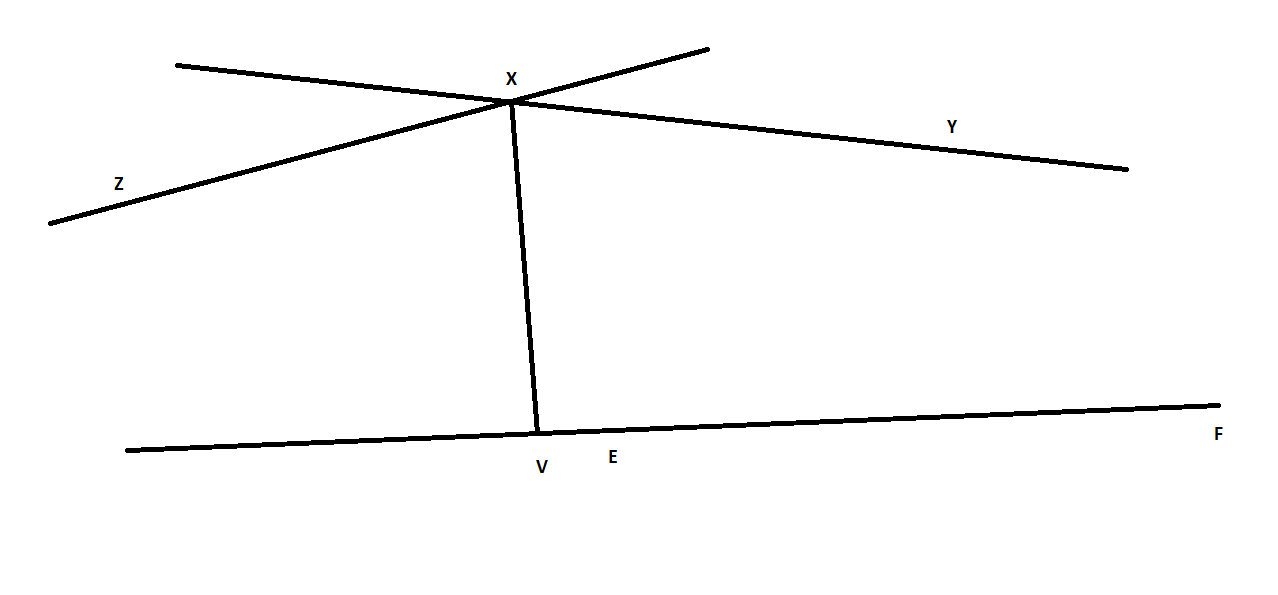
\includegraphics[width=3in]{limitingparallel1.png}
\end{center}

Otherwise we have the case that E*V*F.\\
If $E\in \overrightarrow{XY}$ then $\overrightarrow{XY}$ is not a limiting parallel.  If $\overrightarrow{XY}$ is between $\overrightarrow{XV}$ and $\overrightarrow{XE}$ then by the crossbar theorem is must intersect EV so $\overrightarrow{XY}$ is not a limiting parallel.  Contradiction.\\



Consider U such that $U*E*F$ so we know that $U\not \in \overrightarrow{EF}$.  So U and V are on the same side of $\overleftrightarrow{XY}$ (XY is a limiting parallel to the line U and V are on) and U and Y are on the same side of $\overleftrightarrow{XV}$ (Y and E are on the same side of it, and E and U are on the same side of it).  Therefore $\overrightarrow{XU}$ is between $\overrightarrow{XV}$ and $\overrightarrow{XY}$, so $\overrightarrow{XU}$ must intersect $\overrightarrow{EF}$, but it does not.  Contradiction.  

\begin{center}
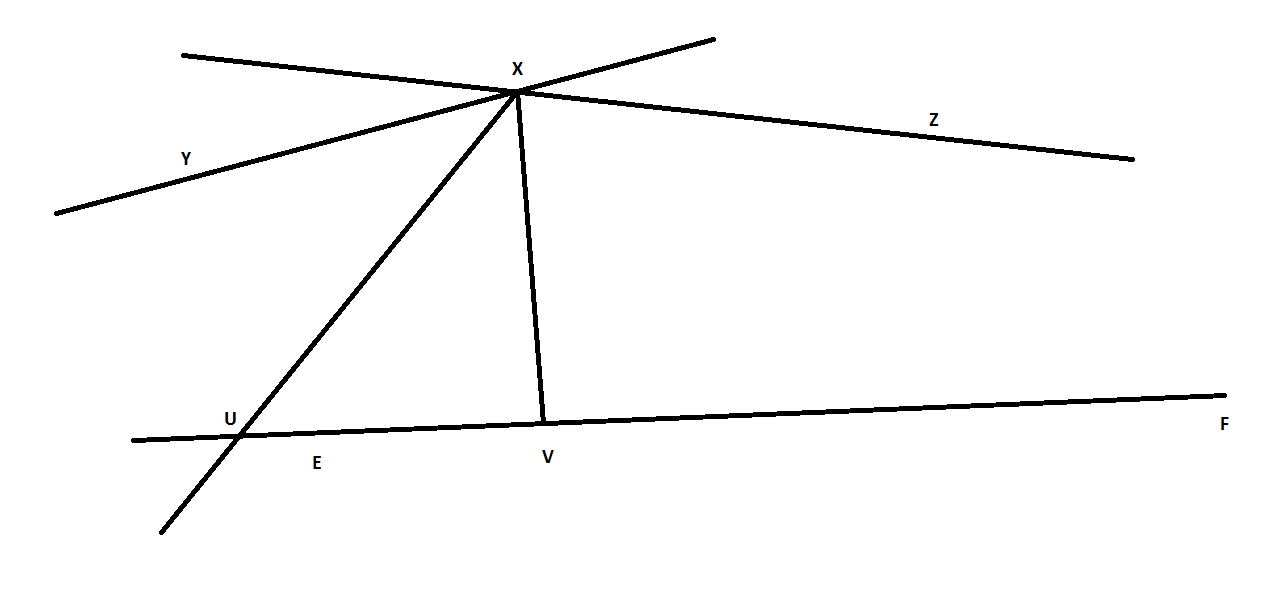
\includegraphics[width=3in]{limitingparallel2.png}
\end{center}


\QED

\newpage 


2. Hence there are two cases depending on whether $\overleftrightarrow{EF}$ is between $\overleftrightarrow{AB}$ and $\overleftrightarrow{CD}$ or $\overleftrightarrow{AB}$ and $\overleftrightarrow{CD}$ are both on the same side of $\overleftrightarrow{EF}$.\\

Since a line divides a plane into two half planes, either both lines can be on the same side of $\overleftrightarrow{EF}$ or on opposite sides.  If they are on the same side, $\overleftrightarrow{EF}$ and $\overleftrightarrow{AB}$ could be on the same side of $\overleftrightarrow{CD}$ or they might not be, however, these are effectively the same case as we currently know no differences between $\overleftrightarrow{AB}$ and $\overleftrightarrow{CD}$.  These leaves us with just the two mentioned cases.\\



3. In the case where $\overleftrightarrow{EF}$ is between $\overleftrightarrow{AB}$ and $\overleftrightarrow{CD}$, let G be the intersection of AC with $\overleftrightarrow{EF}$ (see figure 6.26).  We may assume G lies on ray $\overrightarrow{EF}$; otherwise we can consider $\overrightarrow{GF}$.\\

When we say that $\overleftrightarrow{EF}$ is between $\overleftrightarrow{AB}$ and $\overleftrightarrow{CD}$ we mean that any triplet $(X_1,X_2,X_3) \in (\overleftrightarrow{AB},\overleftrightarrow{EF},\overleftrightarrow{CD})$ has the property that 




4. Any ray $\overrightarrow{AH}$ interior to $\angle GAB$ must intersect $\overrightarrow{EF}$ in a point l.\\

5. $\overrightarrow{IH}$, lying interior to $\angle CIF$, must intersect $\overrightarrow{CD}$\\

6. Hence any ray $\overrightarrow{AH}$ interior to $\angle CAB$ must intersect $\overrightarrow{CD}$, so $\overrightarrow{AB}$ is limiting parallel to $\overrightarrow{CD}$. \\

do we need to do the sub lemma? Gasp!

8. Then AE intersects $\overleftrightarrow{CD}$ in a point G, which we may assume lies on ray $\overrightarrow{CD}$. \\

9. Any ray $\overrightarrow{AH}$ interior to $\angle GAB$ intersects $\overrightarrow{EG}$ in a point I.\\

10.  Since $\overrightarrow{CD}$ enters $\triangle AEI$ at G and does not intersect side EI, it must intersect AI.\\

11. Therefore, $\overrightarrow{CD}$ is limiting parallel to $\overrightarrow{AB}$. \\




\prob{Major Exercises 11 } Let ray r emanating from point P be limiting parallel to line l and let Q be the foot of the perpendicular from P to l (Figure 6.38).  Justify the terminology ``asymptotically parallel'' by proving that for any point R between P and Q there exists a point R' on ray r such that $R'Q' \cong RQ$, where Q' is the foot of the perpendicular from R' to l.  (Hint: Use major exercise 3 and proposition 6.6 to prove the line through R that is asymptotically parallel to l in the opposite direction from r intersects r at a point S.  Show that if T is the foot of the perpendicular from S to l, the point R' obtained by reflecting R across line $\overleftrightarrow{ST}$ is the desired point.)

	Similarly, show that the lines diverge in the other direction.  Use a similar method to prove that the perpendicular dropped one line divergently parallel to another are unbounded. 




\end{document}